% ============================================================
%  Section 4: Results and discussion
% ============================================================
% Every number quoted here is copied from the tables generated by
% experiments/build_paper_assets.py cace (CSV mirrors in results/cace/); none is typed by hand.

\subsection{Evaluation protocol}
\label{subsec:protocol}
All runs start at $\mathbf{x}_{ss}$ with $q_j = \bar q_j$ and use $\Delta t = 0.02$~min. The servo scenarios apply a $-2$~K setpoint step and last $10$~min. Error metrics are computed on the \emph{true} reactor temperature, $\mathrm{IAE} = \int_0^{t_f} |T_{sp} - T|\,dt$, so that sensor noise enters them only through its effect on the valve; ITAE weights the error by the time elapsed since the step. Overshoot $M_p$ (\%) is the peak excursion beyond the setpoint relative to the step size, and the settling time $t_s$ is the last instant at which the error leaves the $\pm 2\%$ band of the step. IAE is reported in K$\cdot$min and ITAE in K$\cdot$min$^2$. The total variation $\mathrm{TV} = |u_0 - \bar q_j| + \sum_k |u_k - u_{k-1}|$ measures valve travel and includes the first move. Because the valve moves at most $1.6$~L/min per sample, TV is bounded by $|u_0 - \bar q_j| + S_{\max} t_f \approx 800$~L/min over $10$~min. The four controllers are AMIGO, Optimal ITAE ($M_s \le 1.6$), NMPC-Oracle and NMPC-MHE (Sections~\ref{sec:formulation}--\ref{sec:baselines}). Noise is Gaussian with standard deviation $\sigma$ on the reactor thermocouple, and, for NMPC-MHE, on the jacket thermocouple as well; all random seeds are fixed.

\subsection{Nominal setpoint tracking}
\label{subsec:nominal}
Table~\ref{tab:classical_benchmark} and Fig.~\ref{fig:classical_benchmark} report the noise-free servo step. Both NMPC variants give identical trajectories ($\mathrm{IAE} = 0.808$~K$\cdot$min, $M_p = 5.2\%$, $\mathrm{TV} = 67.4$~L/min), because with a consistent RK4 model the estimator reconstructs $C_A$ exactly from $T$ and $T_j$. Optimal ITAE reaches $\mathrm{IAE} = 0.827$~K$\cdot$min with $M_p = 2.2\%$ and $t_s = 0.94$~min, and AMIGO $0.925$~K$\cdot$min with $M_p = 9.7\%$. Relative to Optimal ITAE the NMPC lowers the IAE by $2.3\%$ and the settling time from $0.94$ to $0.86$~min, while using $39\%$ more valve travel. Near the design point, where the identified FOPTD model is accurate, an $M_s$-constrained PID with correct anti-windup leaves little for nonlinear prediction to gain.

\begin{figure}[!t]
    \centering
    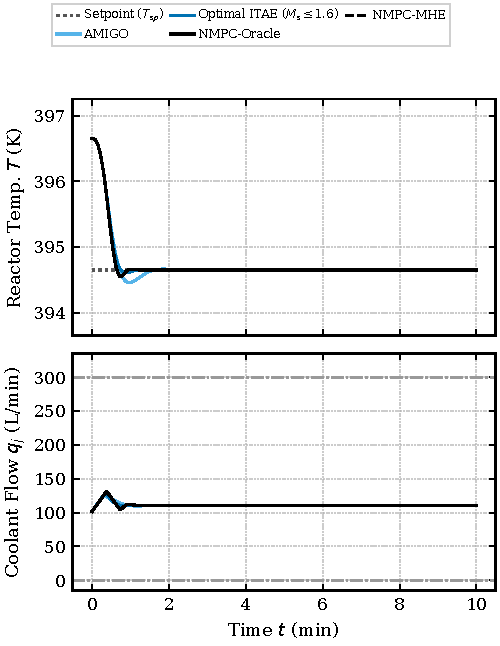
\includegraphics[width=\columnwidth]{figures/fig1_classical_benchmark.pdf}
    \caption{Nominal setpoint tracking ($-2$~K step at $t = 0$, noise-free): reactor temperature $T$ and coolant flow $q_j$ under the valve limits $[0, 300]$~L/min and $80$~L/min$^2$. NMPC-Oracle and NMPC-MHE coincide.}
    \label{fig:classical_benchmark}
\end{figure}

\begin{table*}[t]
\centering
\footnotesize
\caption{Nominal servo benchmark ($-2$~K setpoint step, noise-free) on the non-linear CSTR. FOPTD: $K=-0.1852$~K/(L/min), $\tau=0.6427$~min, $\theta=0.0935$~min. $M_s$ is evaluated on the dead-time FOPTD loop; TV includes the initial valve move from $\bar q_j$.}
\label{tab:classical_benchmark}
\resizebox{\ifdim\width>\textwidth\textwidth\else\width\fi}{!}{%
\begin{tabular}{lcccccccccc}
\toprule
Method & \(K_p\) & \(T_i\text{ (min)}\) & \(T_d\text{ (min)}\) & \(\beta\) & IAE & ITAE (K$\cdot$min$^2$) & TV (L/min) & \(M_p\text{ (\%)}\) & \(t_s\text{ (min)}\) & \(M_s\) \\
\midrule
AMIGO & -17.79 & 0.327 & 0.045 & 1.0 & 0.925 & 0.308 & 40.4 & 9.7 & 1.44 & 1.45 \\
Optimal ITAE ($M_s \leq 1.6$) & -23.55 & 0.465 & 0.032 & 1.0 & 0.827 & 0.204 & 48.6 & 2.2 & 0.94 & 1.60 \\
NMPC-Oracle & -- & -- & -- & -- & 0.808 & 0.190 & 67.4 & 5.2 & 0.86 & -- \\
NMPC-MHE & -- & -- & -- & -- & 0.808 & 0.190 & 67.4 & 5.2 & 0.86 & -- \\
\bottomrule
\end{tabular}%
}
\end{table*}


\subsection{Abrupt fouling event: where nonlinear control pays off}
\label{subsec:nmpc_results}
The decisive scenario combines a $-2$~K setpoint step at $t = 0.5$~min, an abrupt loss of heat transfer to $70\%\,UA$ at $t = 4$~min and thermocouple noise $\sigma = 0.05$~K (Table~\ref{tab:nmpc_oracle_benchmark}, Fig.~\ref{fig:nmpc_oracle}). The fouling event reduces the process gain from $q_j$ to $T$ and raises the coolant demand, so the controllers must move the valve to a new operating point while the reactor heats up.

\begin{figure}[!t]
    \centering
    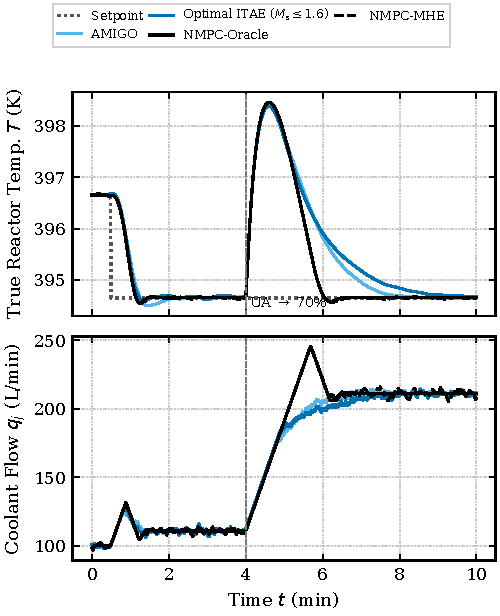
\includegraphics[width=\columnwidth]{figures/fig_nmpc_oracle_comparison.pdf}
    \caption{True reactor temperature and coolant flow under a $-2$~K step at $t = 0.5$~min, abrupt fouling to $70\%\,UA$ at $t = 4$~min (dashed line) and sensor noise $\sigma = 0.05$~K.}
    \label{fig:nmpc_oracle}
\end{figure}

\begin{table*}[t]
\centering
\footnotesize
\caption{Output-feedback gap: NMPC with true-state access (Oracle) vs NMPC with augmented MHE (thermal measurements only) vs $M_s$-constrained PID. $-2$~K step at $t=0.5$~min, jacket fouling to $70\%\,UA$ at $t=4$~min, sensor noise $\sigma=0.05$~K. Both NMPCs: $N=50$ ($1.0$~min), $|\Delta q_j| \le 80\,\Delta t$. Step time is the mean wall-clock time per sample (controller + plant integration; hardware dependent).}
\label{tab:nmpc_oracle_benchmark}
\resizebox{\ifdim\width>\textwidth\textwidth\else\width\fi}{!}{%
\begin{tabular}{lccccccc}
\toprule
Controller & IAE & \(\Delta\)IAE vs Oracle (\%) & ITAE (K$\cdot$min$^2$) & TV (L/min) & \(M_p\) (\%) & \(\hat\alpha_{UA}(t_f)\) & Step time (ms) \\
\midrule
AMIGO & 6.932 & +26.6 & 31.412 & 672.1 & 7.6 & -- & 0.09 \\
Optimal ITAE ($M_s \leq 1.6$) & 7.320 & +33.7 & 34.853 & 694.4 & 3.3 & -- & 0.09 \\
NMPC-Oracle & 5.474 & +0.0 & 23.034 & 252.4 & 5.2 & 0.700 & 31.46 \\
NMPC-MHE & 5.568 & +1.7 & 23.495 & 571.0 & 5.8 & 0.699 & 39.28 \\
\bottomrule
\end{tabular}%
}
\end{table*}


Among the PID loops, AMIGO recovers faster from the loss of cooling ($\mathrm{IAE} = 6.932$~K$\cdot$min) than Optimal ITAE ($7.320$~K$\cdot$min), because it has the larger integral gain ($|K_p|/T_i = 54.4$ versus $50.6$~min$^{-1}$, Table~\ref{tab:classical_benchmark}), at the price of a larger overshoot ($7.6\%$ versus $3.3\%$). The ranking of the nominal step is thus reversed: the tuning that is best for servo tracking is not the best after a change of the plant. NMPC-Oracle reaches $\mathrm{IAE} = 5.474$~K$\cdot$min, i.e. $21.0\%$ below AMIGO and $25.2\%$ below Optimal ITAE when these act on the raw noisy signal. The Oracle reads the noise-free state ($\mathrm{TV} = 252.4$~L/min), so its valve travel is not comparable to that of PID loops fed with noisy measurements and is not used for any travel claim; the symmetric comparison, with a measurement filter on the PID loops, is made in Section~\ref{subsec:deconf}, where the IAE gap to filtered AMIGO shrinks to $13.5\%$ for NMPC-MHE. After the event the estimator identifies the loss of heat transfer, and the NMPC re-plans the coolant trajectory to the new operating point against the rate limit; at $t_f$ the estimate is $\hat\alpha_{UA} = 0.700$ (Oracle) and $0.699$ (MHE) for a true value of $0.70$.

The output-feedback variant stays within $1.7\%$ of the Oracle in IAE ($5.568$~K$\cdot$min), so the two thermal measurements carry enough information to reconstruct both $C_A$ and $\alpha_{UA}$. The price of output feedback appears in the valve travel ($571.0$ versus $252.4$~L/min), which is still below that of both PID loops: the estimator propagates part of the measurement noise into the optimizer's initial state.

\paragraph{Computational cost.} The last column of Table~\ref{tab:nmpc_oracle_benchmark} gives the mean wall-clock time per sample, including the plant integration, measured on a desktop CPU: $31.46$~ms for NMPC-Oracle, $39.28$~ms for NMPC-MHE and $0.09$~ms for each PID loop. The moving-horizon estimator adds about $8$~ms per sample to the NMPC. Both NMPCs are thus several hundred times more expensive than a PID loop, but use less than $4\%$ of the $1.2$~s sampling interval, so real-time feasibility is not the limiting factor on this process. These times are hardware dependent; their ratio, not their absolute value, is the transferable result.

\subsection{Sensitivity of NMPC-MHE to the estimator covariances}
\label{subsec:mhe_tuning}
Table~\ref{tab:mhe_tuning} repeats the NMPC-MHE run of Table~\ref{tab:nmpc_oracle_benchmark} with the measurement covariance $R_e$ and the fouling random-walk variance $Q_\alpha$ scaled by $0.1$ and $10$. The nominal row reproduces Table~\ref{tab:nmpc_oracle_benchmark} ($\mathrm{IAE} = 5.568$~K$\cdot$min, $\mathrm{TV} = 571.0$~L/min).

\begin{table*}[t]
\centering
\footnotesize
\caption{Sensitivity of NMPC-MHE to the estimator covariances on the scenario of Table~\ref{tab:nmpc_oracle_benchmark} (fouling to $70\%\,UA$ at $t = 4$~min, $\sigma = 0.05$~K). $R_e$ is scaled as a whole, $Q_{\alpha}$ is the fouling random-walk variance. Settling: time after the fouling event from which $|\hat\alpha_{UA} - \alpha_{UA}| \le 0.02$ holds until $t_f$.}
\label{tab:mhe_tuning}
\resizebox{\ifdim\width>\textwidth\textwidth\else\width\fi}{!}{%
\begin{tabular}{lccccc}
\toprule
Covariance scaling & IAE & TV (L/min) & RMS \(\hat C_A - C_A\) (mol/L) & \(\hat\alpha_{UA}(t_f)\) & \(\alpha\) settling (min) \\
\midrule
Nominal & 5.568 & 571.0 & 6.97e-05 & 0.699 & 0.14 \\
\(R_e \times 0.1\) & 5.558 & 590.8 & 7.41e-05 & 0.699 & 0.14 \\
\(R_e \times 10\) & 5.574 & 508.8 & 6.18e-05 & 0.699 & 0.14 \\
\(Q_{\alpha} \times 0.1\) & 5.569 & 570.6 & 6.97e-05 & 0.699 & 0.14 \\
\(Q_{\alpha} \times 10\) & 5.567 & 571.7 & 6.97e-05 & 0.699 & 0.14 \\
\bottomrule
\end{tabular}%
}
\end{table*}


Over two decades of each covariance the fouling estimate enters the $\pm 0.02$ band within $0.14$~min of the event and ends at $\hat\alpha_{UA} = 0.699$, the RMS error of $\hat C_A$ stays between $6.18 \times 10^{-5}$ and $7.41 \times 10^{-5}$~mol/L, and the IAE varies only between $5.558$ and $5.574$~K$\cdot$min. $Q_\alpha$ has practically no effect, because the fouling factor is re-estimated at every sample by the moving-horizon refinement rather than propagated by the EKF. $R_e$ acts as a smoothing knob that trades valve travel ($590.8$~L/min for $R_e \times 0.1$, $508.8$~L/min for $R_e \times 10$) against a marginal change in tracking error. On this observable process the estimator does not require fine covariance tuning.

\subsection{Graded fouling and the thermodynamic boundary}
\label{subsec:fouling_results}
Table~\ref{tab:fouling_sensitivity} and Fig.~\ref{fig:fouling_robustness} report a deterministic sweep $UA \in \{100, 90, 80, 70, 60\}\%$ of the nominal value. Every run starts from the clean-jacket steady state, and the reduced $UA$ acts from $t = 0$ together with the setpoint step; the controllers must therefore reject the loss of cooling and track the new setpoint simultaneously. The $100\%$ rows reproduce Table~\ref{tab:classical_benchmark}. The $60\%$ rows are shown for reference only and are excluded from every controller ranking, for the physical reason derived below.

\begin{figure*}[!t]
    \centering
    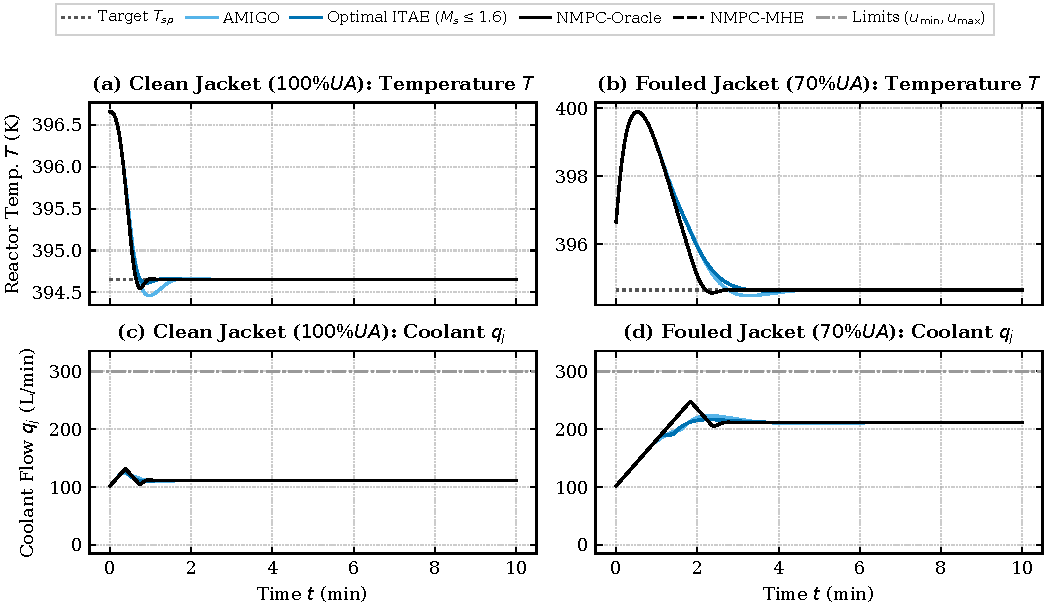
\includegraphics[width=0.98\textwidth]{figures/fig3_fouling_robustness.pdf}
    \caption{Effect of heat-transfer degradation (deterministic, start from the clean-jacket steady state): clean jacket ($100\%\,UA$) versus fouled jacket ($70\%\,UA$).}
    \label{fig:fouling_robustness}
\end{figure*}

\begin{table*}[t]
\centering
\footnotesize
\caption{Impact of heat exchanger fouling ($UA$ reduction from $100\%$ to $60\%$) on closed-loop tracking metrics.}
\label{tab:fouling_sensitivity}
\resizebox{\ifdim\width>\textwidth\textwidth\else\width\fi}{!}{%
\begin{tabular}{lccccc}
\toprule
Method & $UA / UA_{\text{nom}}$ & IAE & ITAE (K$\cdot$min$^2$) & TV (L/min) & $M_p$ (\%) \\
\midrule
AMIGO & 100\% & 0.93 & 0.31 & 40.4 & 9.7 \\
AMIGO & 90\% & 1.75 & 0.78 & 54.4 & 9.7 \\
AMIGO & 80\% & 3.56 & 2.27 & 90.0 & 11.2 \\
AMIGO & 70\% & 7.83 & 7.73 & 147.8 & 8.5 \\
AMIGO & 60\% & 31.08 & 115.44 & 209.1 & 0.0 \\
Optimal ITAE ($M_s \leq 1.6$) & 100\% & 0.83 & 0.20 & 48.6 & 2.2 \\
Optimal ITAE ($M_s \leq 1.6$) & 90\% & 1.72 & 0.71 & 56.8 & 0.0 \\
Optimal ITAE ($M_s \leq 1.6$) & 80\% & 3.48 & 2.06 & 73.1 & 0.1 \\
Optimal ITAE ($M_s \leq 1.6$) & 70\% & 7.76 & 7.44 & 143.0 & 1.4 \\
Optimal ITAE ($M_s \leq 1.6$) & 60\% & 30.79 & 114.60 & 205.8 & 0.0 \\
NMPC-Oracle & 100\% & 0.81 & 0.19 & 67.4 & 5.2 \\
NMPC-Oracle & 90\% & 1.57 & 0.55 & 92.0 & 5.5 \\
NMPC-Oracle & 80\% & 3.19 & 1.67 & 129.5 & 5.7 \\
NMPC-Oracle & 70\% & 6.95 & 5.70 & 196.7 & 4.3 \\
NMPC-Oracle & 60\% & 30.56 & 113.90 & 200.0 & 0.0 \\
NMPC-MHE & 100\% & 0.81 & 0.19 & 67.4 & 5.2 \\
NMPC-MHE & 90\% & 1.57 & 0.55 & 92.0 & 5.5 \\
NMPC-MHE & 80\% & 3.19 & 1.67 & 129.5 & 5.7 \\
NMPC-MHE & 70\% & 6.95 & 5.70 & 196.7 & 4.3 \\
NMPC-MHE & 60\% & 30.56 & 113.90 & 200.0 & 0.0 \\
\bottomrule
\end{tabular}%
}
\end{table*}


The NMPC advantage grows with the mismatch between the plant and the conditions the PID loops were tuned for: at $70\%\,UA$ both NMPC variants give $\mathrm{IAE} = 6.95$~K$\cdot$min against $7.76$ (Optimal ITAE) and $7.83$~K$\cdot$min (AMIGO), $10.4\%$ below the better PID. The gain is smaller than in the fouling event of Section~\ref{subsec:nmpc_results}; a plausible reason is that here the loss of cooling coincides with the setpoint step, so all controllers start the same large valve move at $t = 0$, whereas in the event the PID loops are surprised by the loss of cooling after having settled with a clean jacket.

\paragraph{Thermodynamic loss of controllability at $60\%\,UA$.} At $T_{sp} = 394.65$~K and full cooling there is no steady state at $T_{sp}$ below a critical heat-transfer capacity. At $T = T_{sp}$ the quasi-steady concentration $C_A = qC_{Af}/(q + Vk(T_{sp}))$ fixes the heat release, and the reactor energy balance with the jacket temperature $T_j(\alpha, q_j)$ from the jacket balance gives the residual
\begin{align}
    R(\alpha) &= \tfrac{q}{V}(T_f - T_{sp}) + \tfrac{(-\Delta H)}{\rho C_p}\,k(T_{sp})\,C_A \nonumber \\
    &\quad - \tfrac{\alpha\,UA}{V\rho C_p}\bigl(T_{sp} - T_j(\alpha, q_{j,\max})\bigr), \label{eq:ua_crit} \\
    T_j &= \frac{\tfrac{q_j}{V_j}T_{jf} + \tfrac{\alpha UA}{V_j\rho_jC_{pj}}T_{sp}}{\tfrac{q_j}{V_j} + \tfrac{\alpha UA}{V_j\rho_jC_{pj}}},
\end{align}
which must be $\le 0$ (cooling surplus) with $q_{j,\max} = 300$~L/min for $T_{sp}$ to be reachable. Here $R(1) = -21.2$~K/min and $R(0.6) = +2.44$~K/min, and the root of $R(\alpha) = 0$ is $UA_{\mathrm{crit}} = 63.75\%\,UA_{\mathrm{nom}}$ (Table~\ref{tab:ua_critical}). At $60\%\,UA$ the only equilibrium with the valve fully open, found by scanning $300$--$500$~K, is $396.65$~K $> T_{sp}$. The reported $\mathrm{IAE} = 30.56$--$31.08$~K$\cdot$min and $M_p = 0.0\%$ are therefore the integral of an unavoidable error, with the NMPC travel of exactly $200.0$~L/min being the ramp to the $300$~L/min limit, and not a failure of any control law: no controller acting through this valve can change it.

\begin{table*}[t]
\centering
\footnotesize
\caption{Steady states with the valve fully open ($q_j = 300$~L/min) as a function of $UA$; $T_{sp} = 394.65$~K and $UA_{\mathrm{crit}} = 63.75\%$, the root of the steady-state energy balance at $T=T_{sp}$.}
\label{tab:ua_critical}
\resizebox{\ifdim\width>\textwidth\textwidth\else\width\fi}{!}{%
\begin{tabular}{lcc}
\toprule
\(UA/UA_{\mathrm{nom}}\) & Equilibrium \(T\) at \(q_j = 300\) (K) & Reaches \(T_{sp}\)? \\
\midrule
100.0\% & 377.94 & yes \\
90.0\% & 382.24 & yes \\
80.0\% & 386.71 & yes \\
70.0\% & 391.47 & yes \\
63.7\% (\(UA_{\mathrm{crit}}\)) & 394.65 & yes \\
60.0\% & 396.65 & no \\
\bottomrule
\end{tabular}%
}
\end{table*}


\subsection{Unmeasured feed disturbances: the offset of NMPC and its removal}
\label{subsec:load_results}
Two sequential unmeasured shocks were applied at constant setpoint with $\sigma = 0.05$~K: a feed temperature step $\Delta T_f = +5$~K at $t = 2$~min and a feed concentration step $\Delta C_{Af} = +0.2$~mol/L ($+20\%$) at $t = 8$~min (Table~\ref{tab:load_disturbance}, Fig.~\ref{fig:disturbance_rejection}).

\begin{figure}[!t]
    \centering
    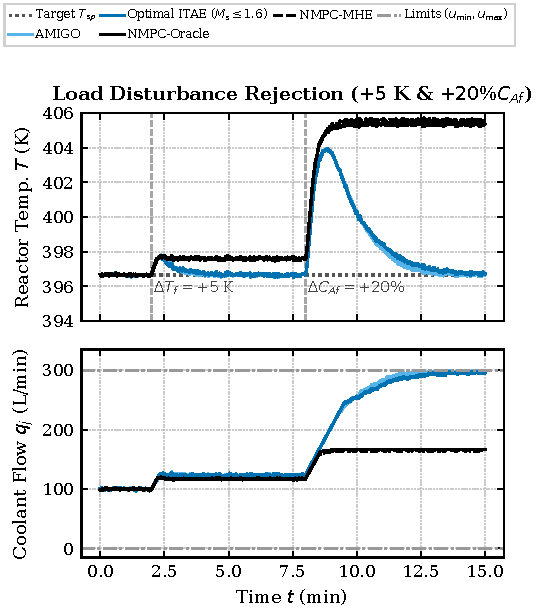
\includegraphics[width=\columnwidth]{figures/fig2_disturbance_rejection.pdf}
    \caption{Unmeasured load disturbances: $+5$~K feed temperature step at $t = 2$~min followed by a $+20\%$ feed concentration step at $t = 8$~min (sensor noise $\sigma = 0.05$~K).}
    \label{fig:disturbance_rejection}
\end{figure}

\begin{table*}[t]
\centering
\footnotesize
\caption{Regulatory performance under combined feed temperature ($+5$~K) and concentration ($+20\%$) load disturbances. $T(t_f) - T_{sp}$ is the true temperature error at $t_f = 15$~min; $\hat\alpha_{UA}(t_f)$ is the NMPC fouling estimate (true value $1.0$, no fouling in this test).}
\label{tab:load_disturbance}
\resizebox{\ifdim\width>\textwidth\textwidth\else\width\fi}{!}{%
\begin{tabular}{lccccccc}
\toprule
Method & IAE & ITAE (K$\cdot$min$^2$) & TV (L/min) & Peak Dev (K) & Max Valve (L/min) & \(T(t_f) - T_{sp}\) (K) & \(\hat\alpha_{UA}(t_f)\) \\
\midrule
AMIGO & 15.27 & 139.03 & 1013.8 & 7.29 & 299.5 & +0.02 & -- \\
Optimal ITAE ($M_s \leq 1.6$) & 16.20 & 150.00 & 1036.5 & 7.28 & 298.8 & +0.07 & -- \\
NMPC-Oracle & 63.91 & 706.75 & 75.9 & 8.82 & 166.6 & +8.69 & 0.981 \\
NMPC-MHE & 65.17 & 722.28 & 511.8 & 9.04 & 165.6 & +8.91 & 0.985 \\
\bottomrule
\end{tabular}%
}
\end{table*}


Both PID loops return to the setpoint ($T(t_f) - T_{sp} = +0.02$~K for AMIGO and $+0.07$~K for Optimal ITAE) with $\mathrm{IAE} = 15.27$ and $16.20$~K$\cdot$min, driving the valve close to its limit ($299.5$ and $298.8$~L/min). The NMPC variants without a disturbance model perform worst ($\mathrm{IAE} = 63.91$ and $65.17$~K$\cdot$min, peak deviation $8.82$ and $9.04$~K) and do not return to the setpoint: at $t_f = 15$~min the error is $+8.69$~K (Oracle) and $+8.91$~K (MHE), with the valve stopped near $166$~L/min.

\paragraph{Diagnosis.} The steady-state energy balance at $T_{sp}$ requires $q_j^\star = 100.0$~L/min for the nominal feed and $297.2$~L/min after both shocks (Table~\ref{tab:horizon_sweep}); the original NMPC stops at $166.6$~L/min, $130.6$~L/min short. A short horizon is not the cause. For $N \in \{30, 50, 75, 100\}$ ($0.6$--$2.0$~min) the final error is $+7.19$, $+8.69$, $+8.78$ and $+8.78$~K: it saturates beyond $N = 75$ instead of vanishing, so the horizon cannot be postponing the action. Fig.~\ref{fig:horizon_diagnosis} shows why. Starting from the realised $T = 405.4$~K, the predicted trajectory crosses $T_{sp}$ after about $0.5$~min, well inside even the shortest horizon, and undershoots it; the optimizer sees no error left to correct while the plant stays $8.7$~K away. The error is in the model:
\begin{figure}[!t]
    \centering
    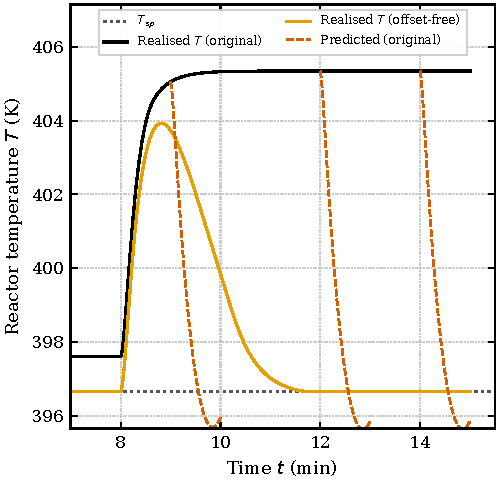
\includegraphics[width=\columnwidth]{figures/fig_horizon_predicted_vs_realised.pdf}
    \caption{Original NMPC-Oracle ($N = 50$): realised temperature and OCP predictions issued at $t = 9, 12$ and $14$~min (dashed), against the offset-free variant. The prediction reaches $T_{sp}$ within the horizon; the plant does not.}
    \label{fig:horizon_diagnosis}
\end{figure}
\begin{enumerate}
    \item \textbf{No disturbance model.} The prediction assumes the nominal $T_f$ and $C_{Af}$. Re-initializing it from the measured or true state at every sample is state feedback, not integral action: the plant is predicted to relax to a temperature that it never reaches, so the optimizer stops moving the valve. Even the Oracle, with perfect state knowledge, keeps the $8.69$~K offset.
    \item \textbf{The estimator absorbs the wrong disturbance.} The only adapted quantity, $\hat\alpha_{UA}$, was introduced for fouling. Under the feed shocks it drifts to $0.981$ (Oracle) and $0.985$ (MHE) although no fouling occurs; this partial compensation is far too small to remove the offset and would raise a false fouling alarm.
    \item \textbf{Remedy.} The integrating disturbance states of Section~\ref{subsec:offset_free}, estimated with the plant states \cite{muske2002disturbance, pannocchia2003disturbance, rawlings2020model}.
\end{enumerate}

\paragraph{Offset-free NMPC.} With Eqs.~\eqref{eq:disturbance_model}--\eqref{eq:disturbance_update}, NMPC-Oracle (OF) returns to the setpoint with $T(t_f) - T_{sp} = 0.00$~K and NMPC-MHE (OF) with $-0.02$~K ($|e_{ss}| < 0.05$~K, also enforced by the unit test of the code), at $\mathrm{IAE} = 12.60$ and $12.84$~K$\cdot$min, $17.5\%$ and $15.9\%$ below AMIGO. The horizon sweep gives the same $297.2$~L/min and zero offset for all four values of $N$. During the $\Delta T_f$ step the estimated $d_T$ settles at $5.000$~K/min $= (q/V)\,\Delta T_f$, as the energy balance requires, and $\hat\alpha_{UA}$ stays at $1.000$ and $1.003$, so the false fouling alarm disappears. The peak deviation ($7.33$ and $7.35$~K) equals that of the PID loops ($7.29$~K): the disturbance is unmeasured and its first effect cannot be prevented. The comparison of Table~\ref{tab:load_disturbance} is therefore now between complete controllers. The valve travel of NMPC-MHE (OF), $876.9$~L/min against $1013.8$~L/min for unfiltered AMIGO, is a comparison with the raw PID signal and is not a symmetric result (Section~\ref{subsec:deconf}).

\begin{table*}[t]
\centering
\footnotesize
\caption{Prediction-horizon sweep of NMPC-Oracle on the feed-disturbance scenario of Table~\ref{tab:load_disturbance}. Steady-state energy balance at $T_{sp}$: $q_j^\star = 100.0$~L/min for the nominal feed and $297.2$~L/min with $\Delta T_f=+5$~K and $\Delta C_{Af}=+20\%$; $T(t_f)-T_{sp}$ is the mean over the last minute.}
\label{tab:horizon_sweep}
\resizebox{\ifdim\width>\textwidth\textwidth\else\width\fi}{!}{%
\begin{tabular}{lcccccc}
\toprule
Variant & \(N\) & Horizon (min) & \(T(t_f)-T_{sp}\) (K) & Valve at \(t_f\) (L/min) & IAE (K$\cdot$min) & Peak dev. (K) \\
\midrule
Original (no disturbance model) & 30 & 0.6 & +7.187 & 182.0 & 55.05 & 8.04 \\
Original (no disturbance model) & 50 & 1.0 & +8.693 & 166.6 & 63.91 & 8.69 \\
Original (no disturbance model) & 75 & 1.5 & +8.783 & 165.7 & 64.42 & 8.78 \\
Original (no disturbance model) & 100 & 2.0 & +8.783 & 165.7 & 64.42 & 8.78 \\
Offset-free & 30 & 0.6 & +0.000 & 297.2 & 12.60 & 7.28 \\
Offset-free & 50 & 1.0 & +0.000 & 297.2 & 12.60 & 7.28 \\
Offset-free & 75 & 1.5 & +0.000 & 297.2 & 12.60 & 7.28 \\
Offset-free & 100 & 2.0 & +0.000 & 297.2 & 12.60 & 7.28 \\
\bottomrule
\end{tabular}%
}
\end{table*}


The original limitation applies to any model-based controller whose model omits the disturbance that actually occurs, not only to the NMPC implemented here.

\subsection{Robustness to sensor noise}
\label{subsec:noise_results}
Table~\ref{tab:noise_sensitivity} and Fig.~\ref{fig:noise_sensitivity} report a Monte Carlo campaign with $30$ noise realizations per level, $\sigma \in \{0.0, 0.1, 0.2, 0.5, 1.0\}$~K, on the nominal servo step ($600$ closed-loop simulations).

\begin{figure}[!t]
    \centering
    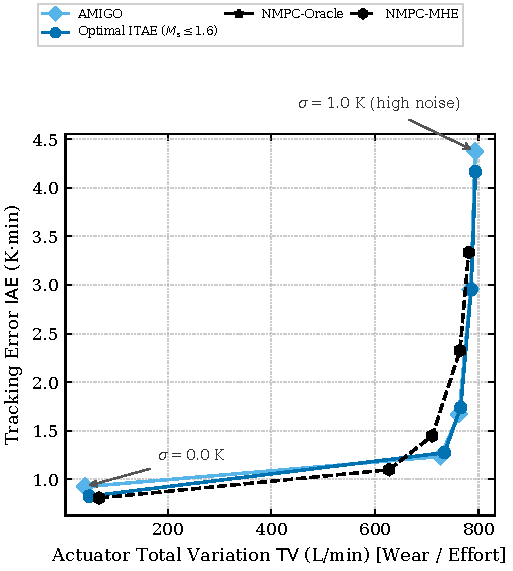
\includegraphics[width=\columnwidth]{figures/fig_noise_sensitivity.pdf}
    \caption{Mean true-temperature tracking error versus mean valve travel as the sensor noise grows from $\sigma = 0$ to $1.0$~K ($30$ Monte Carlo runs per point).}
    \label{fig:noise_sensitivity}
\end{figure}

\begin{table*}[t]
\centering
\footnotesize
\caption{Sensitivity of tracking error (IAE) and actuator effort (TV) to measurement noise levels across $30$ Monte Carlo runs.}
\label{tab:noise_sensitivity}
\resizebox{\ifdim\width>\textwidth\textwidth\else\width\fi}{!}{%
\begin{tabular}{lccc}
\toprule
Method & Noise $\sigma$ (K) & IAE (mean $\pm$ std) & TV (L/min) \\
\midrule
AMIGO & 0.0 & 0.93 $\pm$ 0.00 & 40.4 $\pm$ 0.0 \\
AMIGO & 0.1 & 1.24 $\pm$ 0.05 & 727.0 $\pm$ 7.7 \\
AMIGO & 0.2 & 1.67 $\pm$ 0.14 & 762.2 $\pm$ 6.5 \\
AMIGO & 0.5 & 2.96 $\pm$ 0.46 & 785.0 $\pm$ 5.0 \\
AMIGO & 1.0 & 4.38 $\pm$ 0.92 & 793.5 $\pm$ 1.9 \\
Optimal ITAE ($M_s \leq 1.6$) & 0.0 & 0.83 $\pm$ 0.00 & 48.6 $\pm$ 0.0 \\
Optimal ITAE ($M_s \leq 1.6$) & 0.1 & 1.27 $\pm$ 0.05 & 734.1 $\pm$ 6.8 \\
Optimal ITAE ($M_s \leq 1.6$) & 0.2 & 1.74 $\pm$ 0.12 & 765.5 $\pm$ 6.4 \\
Optimal ITAE ($M_s \leq 1.6$) & 0.5 & 2.95 $\pm$ 0.48 & 785.7 $\pm$ 3.0 \\
Optimal ITAE ($M_s \leq 1.6$) & 1.0 & 4.16 $\pm$ 0.63 & 794.0 $\pm$ 3.3 \\
NMPC-Oracle & 0.0 & 0.81 $\pm$ 0.00 & 67.4 $\pm$ 0.0 \\
NMPC-Oracle & 0.1 & 0.81 $\pm$ 0.00 & 67.4 $\pm$ 0.0 \\
NMPC-Oracle & 0.2 & 0.81 $\pm$ 0.00 & 67.4 $\pm$ 0.0 \\
NMPC-Oracle & 0.5 & 0.81 $\pm$ 0.00 & 67.4 $\pm$ 0.0 \\
NMPC-Oracle & 1.0 & 0.81 $\pm$ 0.00 & 67.4 $\pm$ 0.0 \\
NMPC-MHE & 0.0 & 0.81 $\pm$ 0.00 & 67.4 $\pm$ 0.0 \\
NMPC-MHE & 0.1 & 1.10 $\pm$ 0.04 & 627.6 $\pm$ 10.5 \\
NMPC-MHE & 0.2 & 1.45 $\pm$ 0.09 & 710.7 $\pm$ 9.0 \\
NMPC-MHE & 0.5 & 2.33 $\pm$ 0.22 & 764.2 $\pm$ 6.1 \\
NMPC-MHE & 1.0 & 3.33 $\pm$ 0.26 & 780.9 $\pm$ 5.9 \\
\bottomrule
\end{tabular}%
}
\end{table*}


\begin{enumerate}
    \item \textbf{NMPC-Oracle is invariant to sensor noise} ($\mathrm{IAE} = 0.81 \pm 0.00$~K$\cdot$min, $\mathrm{TV} = 67.4 \pm 0.0$~L/min at every $\sigma$): it reads the true state and feeds its fouling estimator noise-free thermocouples. It shows what an ideal sensor would allow, not what an implementable controller achieves.
    \item \textbf{Output feedback removes the noise immunity of NMPC in valve travel.} At $\sigma = 0.1$~K NMPC-MHE needs $627.6$~L/min against $727.0$ (AMIGO) and $734.1$~L/min (Optimal ITAE); at $\sigma \ge 0.5$~K all three approach the slew-rate ceiling of about $800$~L/min ($764.2$--$794.0$~L/min).
    \item \textbf{NMPC-MHE converts less noise into thermal deviation.} Its IAE grows from $0.81$ to $3.33 \pm 0.26$~K$\cdot$min at $\sigma = 1.0$~K, against $4.16 \pm 0.63$ (Optimal ITAE) and $4.38 \pm 0.92$~K$\cdot$min (AMIGO). The estimator filters the measurement through a physical model, whereas the PID loops act on the raw signal; the derivative filter ($N = 10$) bounds their high-frequency gain at $|K_p|(1 + N)$, which with $|K_p| = 17.79$--$23.55$ still maps $0.1$~K of noise into several L/min per sample.
\end{enumerate}

\subsection{Wide-range multi-point tracking}
\label{subsec:multistep}
A setpoint sequence $396.65 \rightarrow 390.0 \rightarrow 402.0 \rightarrow 396.65$~K over $24$~min with $\sigma = 0.05$~K moves the reactor across operating points with different Arrhenius gains (Table~\ref{tab:multistep_tracking}, Fig.~\ref{fig:multistep_tracking}).

\begin{figure}[!t]
    \centering
    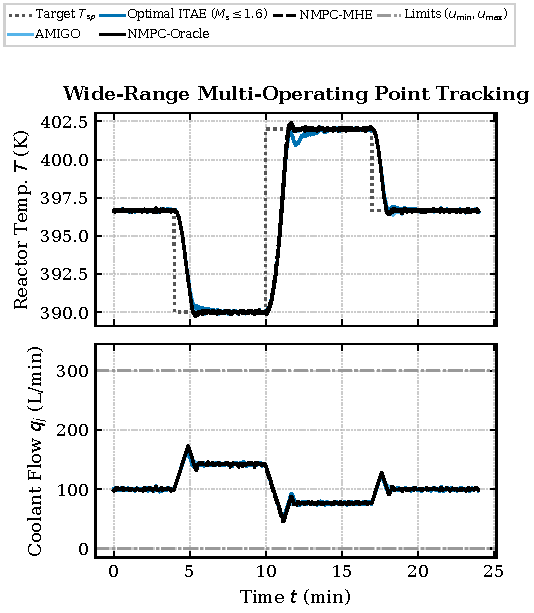
\includegraphics[width=\columnwidth]{figures/fig5_multistep_tracking.pdf}
    \caption{Wide-range setpoint tracking across the moderate ($390.0$~K), nominal ($396.65$~K) and strongly exothermic ($402.0$~K) operating points ($\sigma = 0.05$~K).}
    \label{fig:multistep_tracking}
\end{figure}

\begin{table*}[t]
\centering
\footnotesize
\caption{Multi-operating point tracking across moderate (390~K), nominal (396.65~K), and highly exothermic (402~K) reaction regimes.}
\label{tab:multistep_tracking}
\resizebox{\ifdim\width>\textwidth\textwidth\else\width\fi}{!}{%
\begin{tabular}{lccccc}
\toprule
Method & Total IAE & Total ITAE (K$\cdot$min$^2$) & Total TV (L/min) & Max Valve (L/min) & Min Valve (L/min) \\
\midrule
AMIGO & 20.50 & 208.02 & 1596.7 & 158.4 & 52.7 \\
Optimal ITAE ($M_s \leq 1.6$) & 21.43 & 218.85 & 1650.2 & 166.0 & 48.3 \\
NMPC-Oracle & 19.98 & 201.91 & 388.7 & 173.2 & 46.3 \\
NMPC-MHE & 19.66 & 198.36 & 1221.0 & 173.0 & 45.9 \\
\bottomrule
\end{tabular}%
}
\end{table*}


All controllers remain stable and below saturation (valve range $45.9$--$173.2$~L/min). The error differences are small: AMIGO $20.50$, Optimal ITAE $21.43$, NMPC-Oracle $19.98$ and NMPC-MHE $19.66$~K$\cdot$min, so the Oracle is $2.5\%$ below AMIGO. The difference is valve activity, but only the comparison between signals with the same noise is fair. NMPC-Oracle ($388.7$~L/min) reads the noise-free state and is not comparable to PID loops on the raw measurement ($1596.7$ and $1650.2$~L/min), so no ratio is claimed for it. NMPC-MHE sees the same noise as the PID loops and needs $1221.0$~L/min, $23.5\%$ less than unfiltered AMIGO; Section~\ref{subsec:deconf} shows that a measurement filter on the PID removes this advantage in the fouling transient. NMPC-MHE has a slightly lower IAE than the Oracle here ($19.66$ versus $19.98$~K$\cdot$min); a plausible but untested reason is that the estimator smooths the state fed to the optimizer, while the Oracle reacts to the exact state.

\subsection{De-confounding the NMPC gain: adaptation, nonlinearity, rate planning, mismatch}
\label{subsec:deconf}
The $21\%$ gain of Section~\ref{subsec:nmpc_results} mixes four effects: the PID loops act on a noisy signal, the NMPC re-estimates $\alpha_{UA}$, it predicts with a nonlinear model, and it plans against the slew limit. Table~\ref{tab:deconfounding} repeats the fouling transient with symmetric noise ($\sigma = 0.05$~K on both thermocouples for the NMPC-MHE; a first-order measurement filter, $\tau_f = 0.05$~min, on every PID rule), with all six PID rules rather than the post-hoc choice of AMIGO, with a gain-scheduled PID $K_p = K_{p0}/\hat\alpha_{UA}$ fed by the same estimator, and with NMPC ablations (frozen $\alpha_{UA} = 1$; a planner unaware of the slew limit whose moves are clipped by the valve).

\begin{table*}[t]
\centering
\footnotesize
\caption{De-confounded fouling transient ($-2$~K step, $70\%\,UA$ at $t=4$~min, $\sigma=0.05$~K). All PID rules use a first-order measurement filter ($\tau_f=0.05$~min; raw rows for reference); NMPC-MHE sees the same noise. Reference: filtered AMIGO (ZN reaches a lower IAE only with a large overshoot). Gain scheduling: $K_p=K_{p0}/\hat\alpha_{UA}$ with $\hat\alpha_{UA}$ from the NMPC estimator.}
\label{tab:deconfounding}
\resizebox{\ifdim\width>\textwidth\textwidth\else\width\fi}{!}{%
\begin{tabular}{lcccc}
\toprule
Controller & IAE & TV (L/min) & \(M_p\) (\%) & TV vs filtered AMIGO (\%) \\
\midrule
Ziegler-Nichols + filter & 6.100 & 645.5 & 37.5 & -- \\
Cohen-Coon + filter & 6.815 & 659.4 & 47.0 & -- \\
Tyreus-Luyben + filter & 7.336 & 550.8 & 5.3 & -- \\
AMIGO + filter & 6.439 & 410.8 & 13.8 & -- \\
Skogestad SIMC + filter & 10.429 & 182.9 & 0.2 & -- \\
Opt.\ ITAE + filter & 6.330 & 438.4 & 8.0 & -- \\
AMIGO (raw) & 6.932 & 672.1 & 7.6 & -- \\
Opt.\ ITAE (raw) & 7.320 & 694.4 & 3.3 & -- \\
AMIGO + gain scheduling & 6.225 & 457.6 & 13.9 & -- \\
NMPC-MHE (\(\alpha\) frozen = 1) & 24.578 & 350.4 & 5.6 & +14.7 \\
NMPC-MHE (slew-unaware planner) & 6.237 & 668.3 & 40.5 & -62.7 \\
NMPC-MHE & 5.568 & 571.0 & 5.8 & -39.0 \\
NMPC-MHE (offset-free) & 5.746 & 686.2 & 9.2 & -67.0 \\
NMPC-Oracle & 5.474 & 252.4 & 5.2 & -- \\
\bottomrule
\end{tabular}%
}
\end{table*}


\begin{enumerate}
    \item \textbf{Filtering helps the PID.} Filtered AMIGO improves from $\mathrm{IAE} = 6.932$ to $6.439$~K$\cdot$min and from $672.1$ to $410.8$~L/min of travel. NMPC-MHE ($5.568$~K$\cdot$min) is $13.5\%$ below filtered AMIGO, not $21\%$. Ziegler--Nichols reaches the lowest PID error ($6.100$~K$\cdot$min) with $M_p = 37.5\%$; NMPC-MHE is still $8.7\%$ below it, and below every filtered rule. AMIGO is kept as reference because it was fixed beforehand, not because it is the lowest.
    \item \textbf{Where the gain comes from.} The ladder of Table~\ref{tab:deconfounding_ladder} assigns $24.6\%$ of the $0.871$~K$\cdot$min gap between filtered AMIGO and NMPC-MHE to online adaptation (the gain-scheduled PID obtains it without any optimizer), $-1.4\%$ (none) to nonlinear prediction, and $76.8\%$ to planning against the slew-rate limit. Shares depend on the order of the ladder. Removing adaptation from the NMPC is far more costly than removing it from the PID: with $\alpha_{UA}$ frozen at $1$ the IAE rises to $24.58$~K$\cdot$min, $4.4$ times the adaptive value.
    \item \textbf{Valve travel.} NMPC-MHE uses $571.0$~L/min against $672.1$~L/min for unfiltered AMIGO, $15.0\%$ less; with $23.5\%$ from the wide-range test, the reduction against an unfiltered PID is $15$--$24\%$. Against filtered AMIGO ($410.8$~L/min) NMPC-MHE uses $39\%$ \emph{more}. The travel advantage therefore exists only against an unfiltered PID and is not a property of the NMPC.
    \item \textbf{Cost of the disturbance model.} NMPC-MHE (OF) has $\mathrm{IAE} = 5.746$~K$\cdot$min ($+3.2\%$) and $686.2$~L/min of travel ($+20\%$) in this transient: during fouling $d_T$ and $\hat\alpha_{UA}$ compete for the same thermal signature, which is the price of removing the feed-disturbance offset.
\end{enumerate}

\begin{table*}[t]
\centering
\footnotesize
\caption{Sequential decomposition of the NMPC gain over the best filtered PID in the fouling transient. The shares are order-dependent (ladder), not Shapley values; the last row gives the IAE increase when adaptation is removed from the NMPC itself.}
\label{tab:deconfounding_ladder}
\resizebox{\ifdim\width>\textwidth\textwidth\else\width\fi}{!}{%
\begin{tabular}{lccc}
\toprule
Step & IAE after step & \(\Delta\)IAE & Share of total gain (\%) \\
\midrule
Static PID (AMIGO, filtered) & 6.439 & -- & -- \\
(a) Online adaptation of $\hat\alpha_{UA}$ (gain scheduling) & 6.225 & +0.214 & 24.6 \\
(b) Nonlinear model-based prediction & 6.237 & -0.013 & -1.4 \\
(c) Slew-rate constrained planning & 5.568 & +0.669 & 76.8 \\
NMPC-MHE with frozen $\alpha_{UA}=1$ (adaptation removed from NMPC) & 24.578 & +19.010 & -- \\
\bottomrule
\end{tabular}%
}
\end{table*}


\paragraph{Parametric plant--model mismatch.} A Latin-hypercube Monte Carlo ($N = 28$ points, evaluated in parallel) perturbs the NMPC internal model by $\pm 10\%$ in $E/R$, $k_0$, $\Delta H$, $C_{Af}$ and $T_f$ (the latter as $\pm 10\%$ of $T_f - 273.15$~K) against the nominal plant, in the fouling scenario (Table~\ref{tab:mismatch_mc}). In two samples (9 and 21) the perturbed model has no steady state at $q_j = 100$~L/min and the controller cannot be built; they are reported as non-converged, not replaced. In the remaining $26$, the original NMPC-MHE degrades from $\mathrm{IAE} = 5.568$ to a mean of $31.25$ (P95 $94.34$, maximum $101.02$)~K$\cdot$min with a mean steady-state error of $3.59$~K (maximum $12.04$~K); the offset-free variant has a mean $\mathrm{IAE} = 6.41$ (P95 $8.40$) and $|e_{ss}| \le 0.003$~K. The $\pm 10\%$ error in $E/R$ changes $k$ at $T_{sp}$ by a factor of about $9$, a severe mismatch; with $26$ samples the tail percentiles are coarse, and only the model, not the PID, was perturbed.

\begin{table*}[t]
\centering
\footnotesize
\caption{Parametric plant-model mismatch: Latin-hypercube Monte Carlo ($N=28$) of $\pm10\%$ errors of the NMPC internal model in $E_a/R$, $k_0$, $\Delta H$, $C_{Af}$ and $T_f$ (the latter as $\pm10\%$ of $T_f-273.15$~K) against the nominal plant, fouling scenario of Table~\ref{tab:deconfounding}.}
\label{tab:mismatch_mc}
\resizebox{\ifdim\width>\textwidth\textwidth\else\width\fi}{!}{%
\begin{tabular}{lccccccc}
\toprule
Controller & Nominal IAE & IAE mean & IAE P95 & IAE max & \(|e_{ss}|\) mean (K) & \(|e_{ss}|\) max (K) & Converged \\
\midrule
NMPC-MHE (original) & 5.568 & 31.248 & 94.340 & 101.020 & 3.589 & 12.044 & 26/28 \\
NMPC-MHE (offset-free) & 5.746 & 6.414 & 8.399 & 8.503 & 0.002 & 0.003 & 26/28 \\
AMIGO + filter (nominal, no model) & 6.439 & -- & -- & -- & 0.006 & -- & -- \\
\bottomrule
\end{tabular}%
}
\end{table*}


\subsection{When and why nonlinear control outperforms robust PID}
\label{subsec:when_why}
The six scenarios separate the effect of the model from that of the information available to the controller. Nonlinear prediction pays off when the plant leaves the neighbourhood in which the PID was tuned and the change is represented in the model: after the fouling event, a fixed linear controller is tuned for one process gain, and Bode's sensitivity integral \cite{stein2003respect} forces any reduction of $|S(j\omega)|$ at low frequency to be paid by amplification elsewhere, so a single gain cannot be both fast and robust across the gain variation induced by fouling and by the Arrhenius term. Section~\ref{subsec:deconf} shows that the part of this advantage that does not depend on a PID filter comes from updating $\hat\alpha_{UA}$ (which a gain-scheduled PID also captures) and, mostly, from planning the valve ramp against the rate limit, not from the nonlinearity of the model. Where the plant stays near the design point, or the disturbance is not represented in the model, the PID loops are equal or better, and integral action, not prediction, is what decides regulation; with an integrating disturbance model the NMPC regains that property. Neither class of controller crosses the boundary set by the heat-removal capacity of the jacket. Section~\ref{sec:conclusion} condenses these observations into five criteria.

\paragraph{Limitations.} The study uses one reactor, one valve and one fouling magnitude for the estimator study; the plant and the NMPC share the same model structure, so the results bound the benefit of NMPC under structural model match and parametric (fouling) mismatch only. The step times were measured on a single desktop computer. The mismatch study perturbs only the NMPC model and uses $28$ points; the PID loops with setpoint weighting were not part of the symmetric-noise comparison, and the multi-point test was not repeated with filtered PID loops.
